\documentclass{article}

\usepackage{fullpage}
\usepackage{graphicx}
\usepackage{indentfirst}
\usepackage{hyperref}
\hypersetup{
    colorlinks=true,
    urlcolor=blue
}

\usepackage{float}

\title{CSCI 4511W Writing Assignment 1}
\author{Brian Cooper \\ coope824@umn.edu \\ University of Minnesota}
\date{\today}

\begin{document}
\maketitle

\section{Introduction}
In this assignment, some algorithms are tested on two different puzzles (\textit{eight-puzzle} and \textit{n-queens}, described in more detail in their respective sections). An analysis of the resulting algorithm performance is compared.

\section{Eight-Puzzle Problem}

An \textit{eight-puzzle} problem involves a 3x3 board of tiles in which eight of the nine tiles have a number (1-8) on them and one tile is blank (an empty space). The tiles are in a random initial configuration, and the goal is to move the tiles to reach some final tile configuration. Two algorithms, breadth-first search and depth-limited search (with limit 50), were attempted on this problem using code implemented from the \textit{Artificial Intelligence - A Modern Approach} GitHub repository at \url{https://github.com/aimacode/aima-python}.
\\\
\begin{center}
    A comparison of the runtime and memory usage of each approach is outlined in the table below:
\end{center}

    % table for eight puzzle problem
    \begin{table}[H]
        \centering
        \begin{tabular}{c|c|c|}
        \cline{2-3}
                                                              & Time (seconds) & Memory (kilobytes) \\ \hline
        \multicolumn{1}{|c|}{Breadth-First Search}            & 23.457    & 1,662,128      \\ \hline
        \multicolumn{1}{|c|}{Depth-Limited Search (limit 50)} & 12.823    &   99,080      \\ \hline
        \end{tabular}
    \end{table}

These tests were performed on a CSE labs machine in Keller 4-250 at University of Minnesota, using Python scripts to call the algorithms with the following initial configuration:

    \begin{table}[H]
        \centering
        \begin{tabular}{|c|c|c|}
        \hline
        6 & 2 & 3 \\ \hline
        1 & 5 & 4 \\ \hline
          & 7 & 8 \\ \hline
        \end{tabular}
    \end{table}

As mentioned previously, both breadth-first search and depth-limited search (limit = 50) were applied to this problem and initial configuration. Based on the results in the table, depth-limited search was able to complete the puzzle in both less time (almost half) and less memory than breadth-first search; depth-limited search has better time and space complexity than breadth-first search \textbf{on these test simulations}. However, breadth-first search has the advantage of guaranteeing the finding of a solution if it exists (which it does, for this problem). Depth-limited search is only correct if the solution does not exceed the depth limit.
\\
\par The traditional depth-first search algorithm (not limited) is not highly applicable to this problem, since it is not correct (may not find the solution).

\section{N-Queens Problem}

An \textit{n-queens} problem involves an $n \times n$ Chess board. To solve the problem, a configuration in which $n$ queens can be placed on an $n \times n$ board without the ability to attack each other needs to be found.
\\
\par Breadth-first search and depth-first search (not limited) were performed on this problem. Breadth-first search was tested with $n$ values of $\{8, 9, 10, 11, 12, 13\}$, and depth-first search was tested with $n$ values of $\{8, 9, 10, 11, 12, 13, 14, 15, 16, 17, 18, 19, 20\}$.
\\
\begin{center}
    A comparison of the runtime between each approach is outlined below:
\end{center}

    \begin{figure}[H]
      \centering
      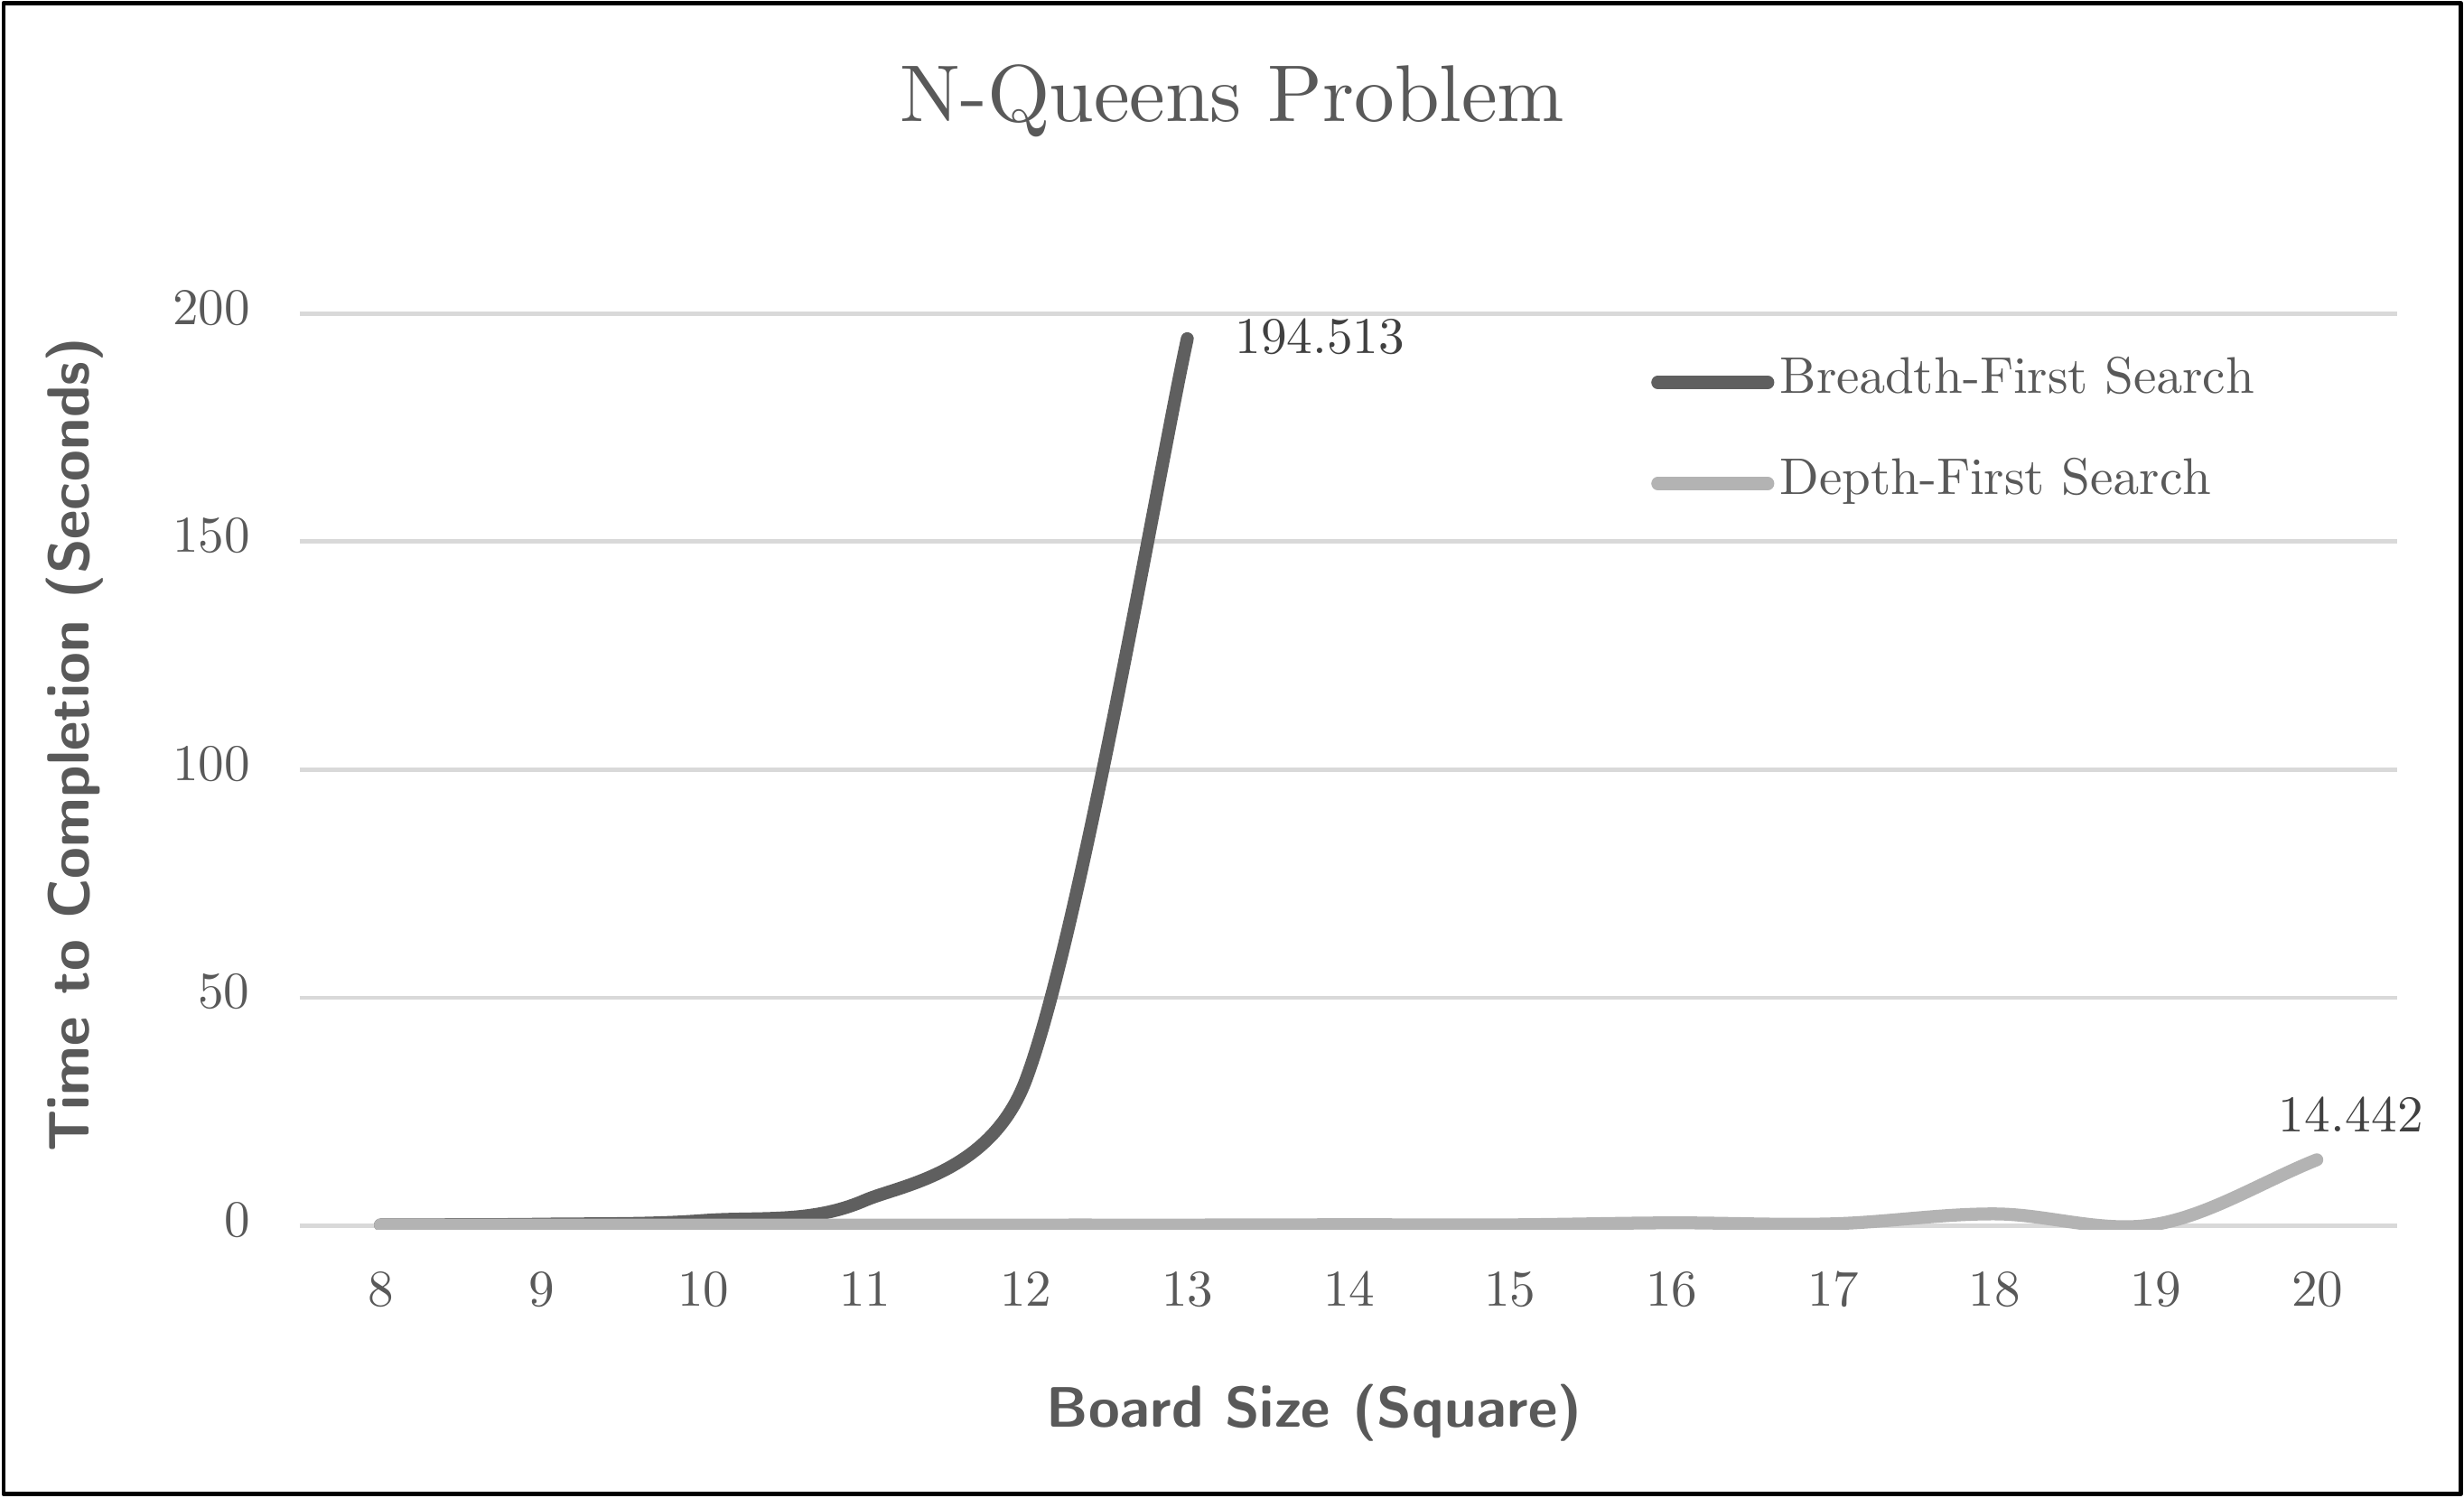
\includegraphics[width=1\textwidth]{figure.png}
    %   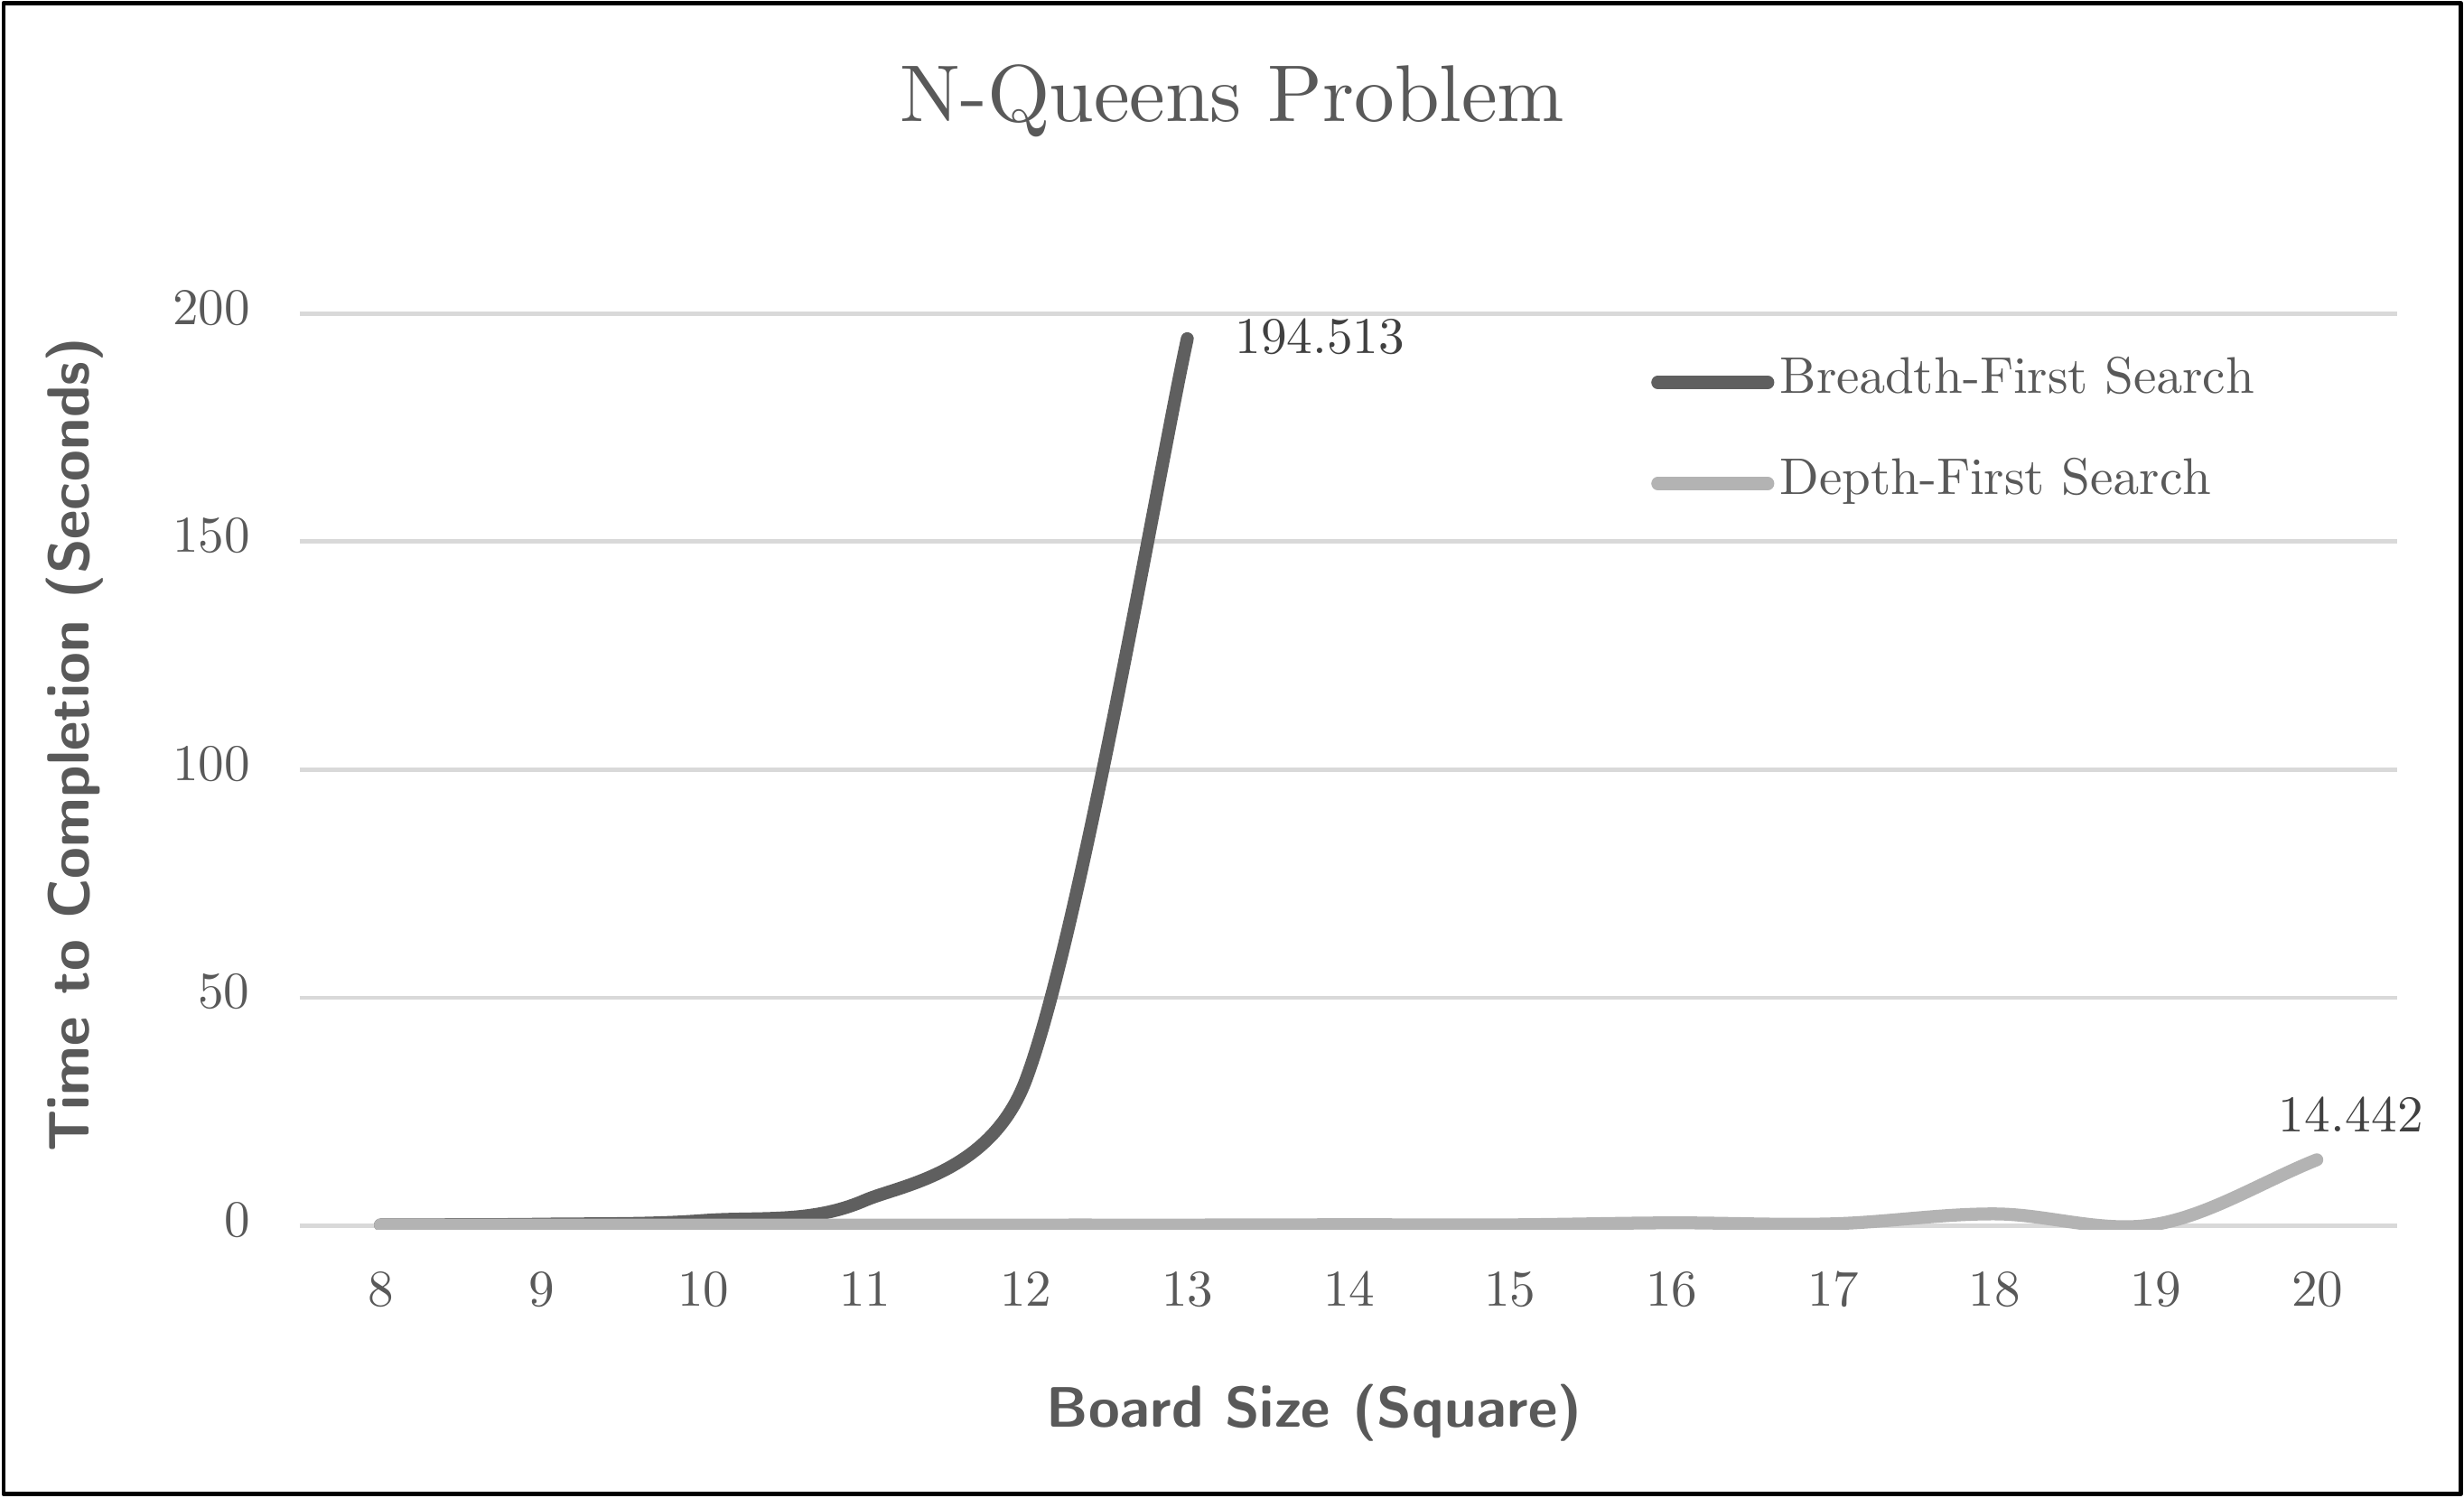
\includegraphics[width=14cm, height=8cm]{figure.png}
      \caption{BFS and DFS approach to N-Queens problem}
    \end{figure}

    As the graph shows, depth-first search performed faster than breadth-first search (even beyond the final test of a $13 \times 13$ board for breadth-first search). Even on the lower limit of these test board sizes, an $8 \times 8$ board, depth-first search completed the problem in approximately 0.136 seconds, while breadth-first search completed the problem in approximately 0.151 seconds. Although close, depth-first search still was able to solve the problem in less time. It was also able to complete larger board sizes before a noticeable spike in duration was reached. Similar to the eight-puzzle problem, depth-first search used less memory than breadth-first search did. Depth-first search with $n=20$ used approximately 99,080 kB, while breadth-first search with $n=8$ used approximately  99,336 kB. Thus, depth-first search has better time and space complexity than breadth-first search \textbf{on these test simulations}. However, as with the previous eight-puzzle problem, breadth-first search has the advantage of guaranteeing the discovery of a solution, whereas depth-first search cannot promise this.

\end{document}
